\documentclass[a4paper]{article}
\usepackage[english]{babel} % for english wordwrapping
% \usepackage{a4wide} % for a4 paper and images
\usepackage[parfill]{parskip} % no indents on new par, but new lines
\usepackage{titling} % for a subtitle
\usepackage{graphicx} % for graphics
% \usepackage{changepage} %adjust width
% \usepackage[official]{eurosym}
% \usepackage{pdfpages} % for the title page
\usepackage[ttscale=.875, ]{libertine} % or any other font package
% \usepackage{etoolbox} % for quotes
% \usepackage{tikz} % for quotes
% \usepackage{xspace} % for space after FixedFoot invocation
\usepackage[colorlinks=true, linkcolor=black, urlcolor=black, citecolor=black]{hyperref} % for urls or internal links
\usepackage{datetime} % month-year
\usepackage[center, sc, compact]{titlesec}
\usepackage{amssymb}

\newcommand{\subtitle}[1]{%
  \posttitle{%
    \par\end{center}
    \begin{center}\Large#1\end{center}
    \vskip0.5em}%
}

\newdateformat{monthdate}{\monthname[\THEMONTH] \THEYEAR}

\title{KLEIN cipher, optimised for high speed}
\subtitle{Cryptographic Engineering -- Assignment 1}
\date{\monthdate\today}
\author{Koen van Ingen, s4058038\\
Joost Rijneveld, s4048911}

\begin{document}

\maketitle

In this report, we describe our implementation of the KLEIN-64 cipher~\cite{gong2012klein} (optimised for high speed) on the AVR ATTiny45 microcontroller. The ATTiny45 is an 8-bit processor that has 32 registers, 512 bytes SRAM and 4096 bytes Flash memory. As it uses 16-bit addresses, addressing memory requires two 8-bit registers. It is worth mentioning that only register 30 and 31 can be used to load from Flash memory.

\section{The KLEIN cipher}
% 1a4 ofzo? diagrammetje? dat het eigenlijk AES is

The KLEIN cipher is a lightweight block cipher that shows many similarities with the Rijndael (AES) cipher. KLEIN consists of roughly the same five operations: AddRoundKey, SubNibbles, RotateNibbles, MixNibbles and KeySchedule. The main difference with AES is the fact that KLEIN operates on nibbles rather than bytes. We will now briefly describe these operations. See \hyperlink{appendix}{the appendix} for a visualisation.

\begin{description}
	\item[AddRoundKey] This operation consists of xoring the round key into the state.
	\item[SubNibbles] In this step, the state is passed through the sbox, one nibble at a time.
	\item[RotateNibbles] This operation rotates the state to the left by four nibbles.
	\item[MixNibbles] This step consists of a series of permutations that can be represented as two matrix multiplications over a finite field. It operates on pairwise concatenations of nibbles as elements of an input vector, effectively mimicking the Rijndael MixColumn operation on bytes.
	\item[KeySchedule] This operation computes the next round key by performing several shifts, sbox lookups and xor operations.
\end{description}

\section{Our implementation}
% memory layout, register layout
% klein zinnetje over c-implementatie

To run our implementation of the KLEIN cipher with a different input, change line 6 to 13 and line 28 to 35 according to the key and plaintext values. The initial key and plaintext are loaded into registers using \texttt{ldi} instructions, and the resulting ciphertext ends up in register 16 to 23. During the execution of the program we keep the round key in register 0 to 7, while the state is alternately in register 8 to 15 and register 16 to 23 depending on the parity of the round (discussed later).

We will now briefly discuss the optimisations we have implemented.

% \subsection{Major optimisations}

\subsection*{Squaring the sbox}

The sbox as presented in the KLEIN paper operates on nibbles, but our state is stored in 8-bit registers. Additionally, loading from memory always returns a full byte of data. As all nibbles are sequentially passed through the sbox during the SubNibbles step, we can also pass them pairwise (as bytes). This requires an sbox that operates on bytes, which can be constructed by squaring the original 8 byte sbox to 256 bytes. By storing this sbox at \texttt{0x0500}, we can conveniently perform two lookups at once by copying a complete state register to the lower half of the address.

\subsection*{Lookup tables for MixNibbles}

The MixNibbles step requires matrix multiplication in $\mathbb{F}_{2^8}$ (modulo $x^4 + 1$). As this would be quite a bit of computation, we have replaced this by lookup tables. KLEIN only uses multiplications by \texttt{0x01}, \texttt{0x02} and \texttt{0x03}, so replacing these operations requires only two 256-byte tables. Since AES uses the same polynomial and multiplication matrices, these lookup tables are readily available. In accordance with their label in the code, we will refer to these tables as \texttt{mult2} and \texttt{mult3} from now on.

\subsection*{Unrolling the loop}

The KLEIN cipher repeats the five aforementioned operations in twelve rounds. To implement such a loop in AVR assembly, we would need to compare the loop index with \texttt{0x0C} at the end of every iteration, and possibly jump back to the beginning of the loop. In order to do this, we also need to maintain and increment the loop index, at the cost of a register and an instruction. By unrolling the loop, we can prevent these expensive jumps and comparisons. We still need the loop index for the KeySchedule operation, but we can now hard code this value and free a register.

\subsection*{Rotating by renaming}

Several registers are rotated in both in the SubNibbles and the KeySchedule operation. Naively, this would result in multiple \texttt{mov} instructions, but all of these can be prevented by implicitly renaming registers. It requires some extra administration, although this can be largely simplified by combining rotation with loading to and from memory. The fact that all our \texttt{mov} operations move to register 30 are a testament to this. This optimisation is largely made possible by unrolling the loop: after unrolling, the parts of the key no longer have to be in the same registers at the end of every round in order to make the next round fit, but can be implicitly renamed.

\hypertarget{lpmtheneor}{}
\subsection*{MixNibbles: \texttt{lpm} then \texttt{eor}}

After passing the state registers through the \texttt{sbox}, it seems to make sense to copy the results to the new state registers immediately. However, by doing this, state registers that are then passed through \texttt{mult2} need to be loaded into a temporary register before being added onto the new state registers using an \texttt{eor} instruction. By first doing the \texttt{lpm} instructions to load the results of \texttt{mult2} to the new state registers (saving eight \texttt{eor}s), we no longer need to copy the \texttt{sbox} results and can use the saved \texttt{eor} instructions here instead. This saves eight \texttt{mov} instructions per round for a grand total of 96 cycles.

\subsection*{The order of \texttt{mult2} and \texttt{mult3} in MixNibbles}

Naively, one would first pass the leftmost half of the state through \texttt{mult2} and \texttt{mult3} and then pass the rightmost half through \texttt{mult2} and \texttt{mult3}. By reversing the order of the last two lookups (so that it becomes \texttt{m2-m3-m3-m2}), we can save one `\texttt{ldi} \texttt{high(mult3} \texttt{*} \texttt{2)}' instruction per round (see line 127).

Intuitively one might try to rearrange it to \texttt{m2-m2-m3-m3} in an attempt to save two such \texttt{ldi} instructions. However, as the pairs of \texttt{m2-m3} and \texttt{m3-m2} operate on the same parts of the state, we can rearrange the `\texttt{mov} \texttt{r30}' instructions so that we can reuse these as well, saving another two instructions per round (see e.g. line 86 and 144).

\subsection*{Merging SubNibbles and MixNibbles}

A similar trick can be applied to combine a \texttt{mov} instruction of the SubNibbles step with the MixNibbles. However, this is not as straightforward as it may appear, as SubNibbles operates on state registers that have not yet been passed through the \texttt{sbox}. By combining the \texttt{sbox} with the \texttt{mult2} and \texttt{mult3} tables, we can make sure that both tables take the same type of input. The \texttt{sbox} table now effectively serves the purpose of a \texttt{mult1} operation.

However, this introduces a problem. As we first passed every state register through the \texttt{sbox} before starting to build the new state, this effectively allowed us to do a `free' move from register 8 to 15 to register 16 to 23. As we would then construct the new state in register 8 to 15, the position of the state was invariant at the end of every round. After combining the lookup tables, this is no longer the case.

This problem can be solved by dividing the rounds in two types: `regular' rounds and `mirrored' rounds. `Regular' rounds transfer the state from the lower registers to the higher ones, while the `mirrored' rounds do exactly the opposite. This also requires two flavours of the AddRoundKey macro.

Now we can finally apply the reordering optimisation, arranging the lookups in such a way that either a `\texttt{ldi} \texttt{high}' or a `mov r30' instruction is saved between every table. An ordering that achieves this is 
\texttt{m2-m1-m3-m3-m2-m1}. This seemingly weird ordering is influenced by the fact that it cannot start with \texttt{m1} (see the \hyperlink{lpmtheneor}{``\texttt{lpm} then \texttt{eor}''} optimisation), but should preferably end in \texttt{m1} to enable the following optimisation.

\subsection*{Prevent \texttt{ldi} \texttt{high} in KeySchedule}

Part of the KeySchedule operation includes passing two bytes through the \texttt{sbox}. Because we made sure to end the ordering of lookup tables with \texttt{m1}, the high part of the address of the sbox is still in \texttt{r31}. This means we do not have to load it again in the KeySchedule operation, saving another 12 cycles.
\newpage
\section{Results}
% beargumenteren waarom dit niet sneller kan
% testvectors werken
% uiteindelijk aantal cycles en bytes in gebruik noemen (misschien tov oude )
% vergelijken met de bestaande AVR-implementatie van klein80 (domme poging tot corrigeren)

First and foremost, it is worth mentioning that the test vectors (as presented in the KLEIN paper) all work correctly for our implementation. For reference, the test vectors are listed below.

\vspace{0.5em}
\begin{center}
	\begin{tabular}{c | c | c}
		\hline
		Key & Plaintext & Ciphertext \\
		\hline
	{\tt \small 0000 0000 0000 0000} & {\tt \small FFFF FFFF FFFF FFFF} & {\tt \small CDC0 B51F 1472 2BBE} \\
	{\tt \small FFFF FFFF FFFF FFFF} & {\tt \small 0000 0000 0000 0000} & {\tt \small 6456 764E 8602 E154} \\
	{\tt \small 1234 5678 90AB CDEF} & {\tt \small FFFF FFFF FFFF FFFF} & {\tt \small 5923 56C4 9971 76C8} \\
	{\tt \small 0000 0000 0000 0000} & {\tt \small 1234 5678 90AB CDEF} & {\tt \small 629F 9D6D FF95 800E} \\
		\hline
	\end{tabular}
\end{center}
\vspace{0.5em}

The table below lists the cycle count of our implementation, as well as the number of bytes of memory our implementation requires. Note that we did not limit the memory usage at all (if it would come at the cost of cycles), as long as the code would fit.

\vspace{0.5em}
\begin{center}
	\begin{tabular}{l r | l r}
		\hline
		Cycle count & \textbf{1748} & Bytes in Flash & \textbf{2916} \\
		\hspace{1em} \emph{\dots for initialisation} & \emph{24} & \hspace{1em} \emph{\dots for the code} & \emph{2148} \\
		\hspace{1em} \emph{\dots per round (12 rounds)} & \emph{143} & \hspace{1em} \emph{\dots for lookup tables} & \emph{768} \\
		\cline{3-4}
		\hspace{1em} \emph{\dots for final AddRoundKey} & \emph{8} & Bytes in SRAM & \textbf{0} \\
		\hline
	\end{tabular}
\end{center}
\vspace{0.5em}

It is perhaps worth mentioning that the authors of the KLEIN paper have provided an AVR-assembly implementation~\cite{eisenbarth2012compact}. Their implementation uses 80-bit keys and runs in \texttt{6095} clock cycles. A 64-bit port of this implementation runs in \texttt{4622} cycles. To be fair, this implementation was largely optimised for minimal size (although some optimisations for speed were included), making a speed comparison a bit biased.

\subsection*{Rejected `optimisations'}

One of the popular implementation optimisations of the Rijndael cipher is to create so-called Tbox lookup tables to speed up the MixColumns step and combine it with SubBytes. However, this approach is not feasible for the AVR processor, as memory is loaded in chunks of 8 bits while 32 bits are required for this to work effectively. Additionally, constructing four of these tables would not fit in memory (as they are 1KB each), and rotating just one table would be very expensive.

Another approach can be to interleave the current lookup tables, in order to prevent having to reload the address and to be able to continuously lookup multiplication results using post increment. However, this makes addressing much harder, as one has to dynamically double the addresses (requiring several extra cycles).

% considerations: Tboxen zoals AES, Z+ to combine tables,

\bibliographystyle{unsrt}
\bibliography{bibliography}

\appendix

\hypertarget{appendix}{}
\section*{Appendix:\hspace{1em}Diagram of the KLEIN cipher}

\begin{center}
  \makebox[\textwidth]{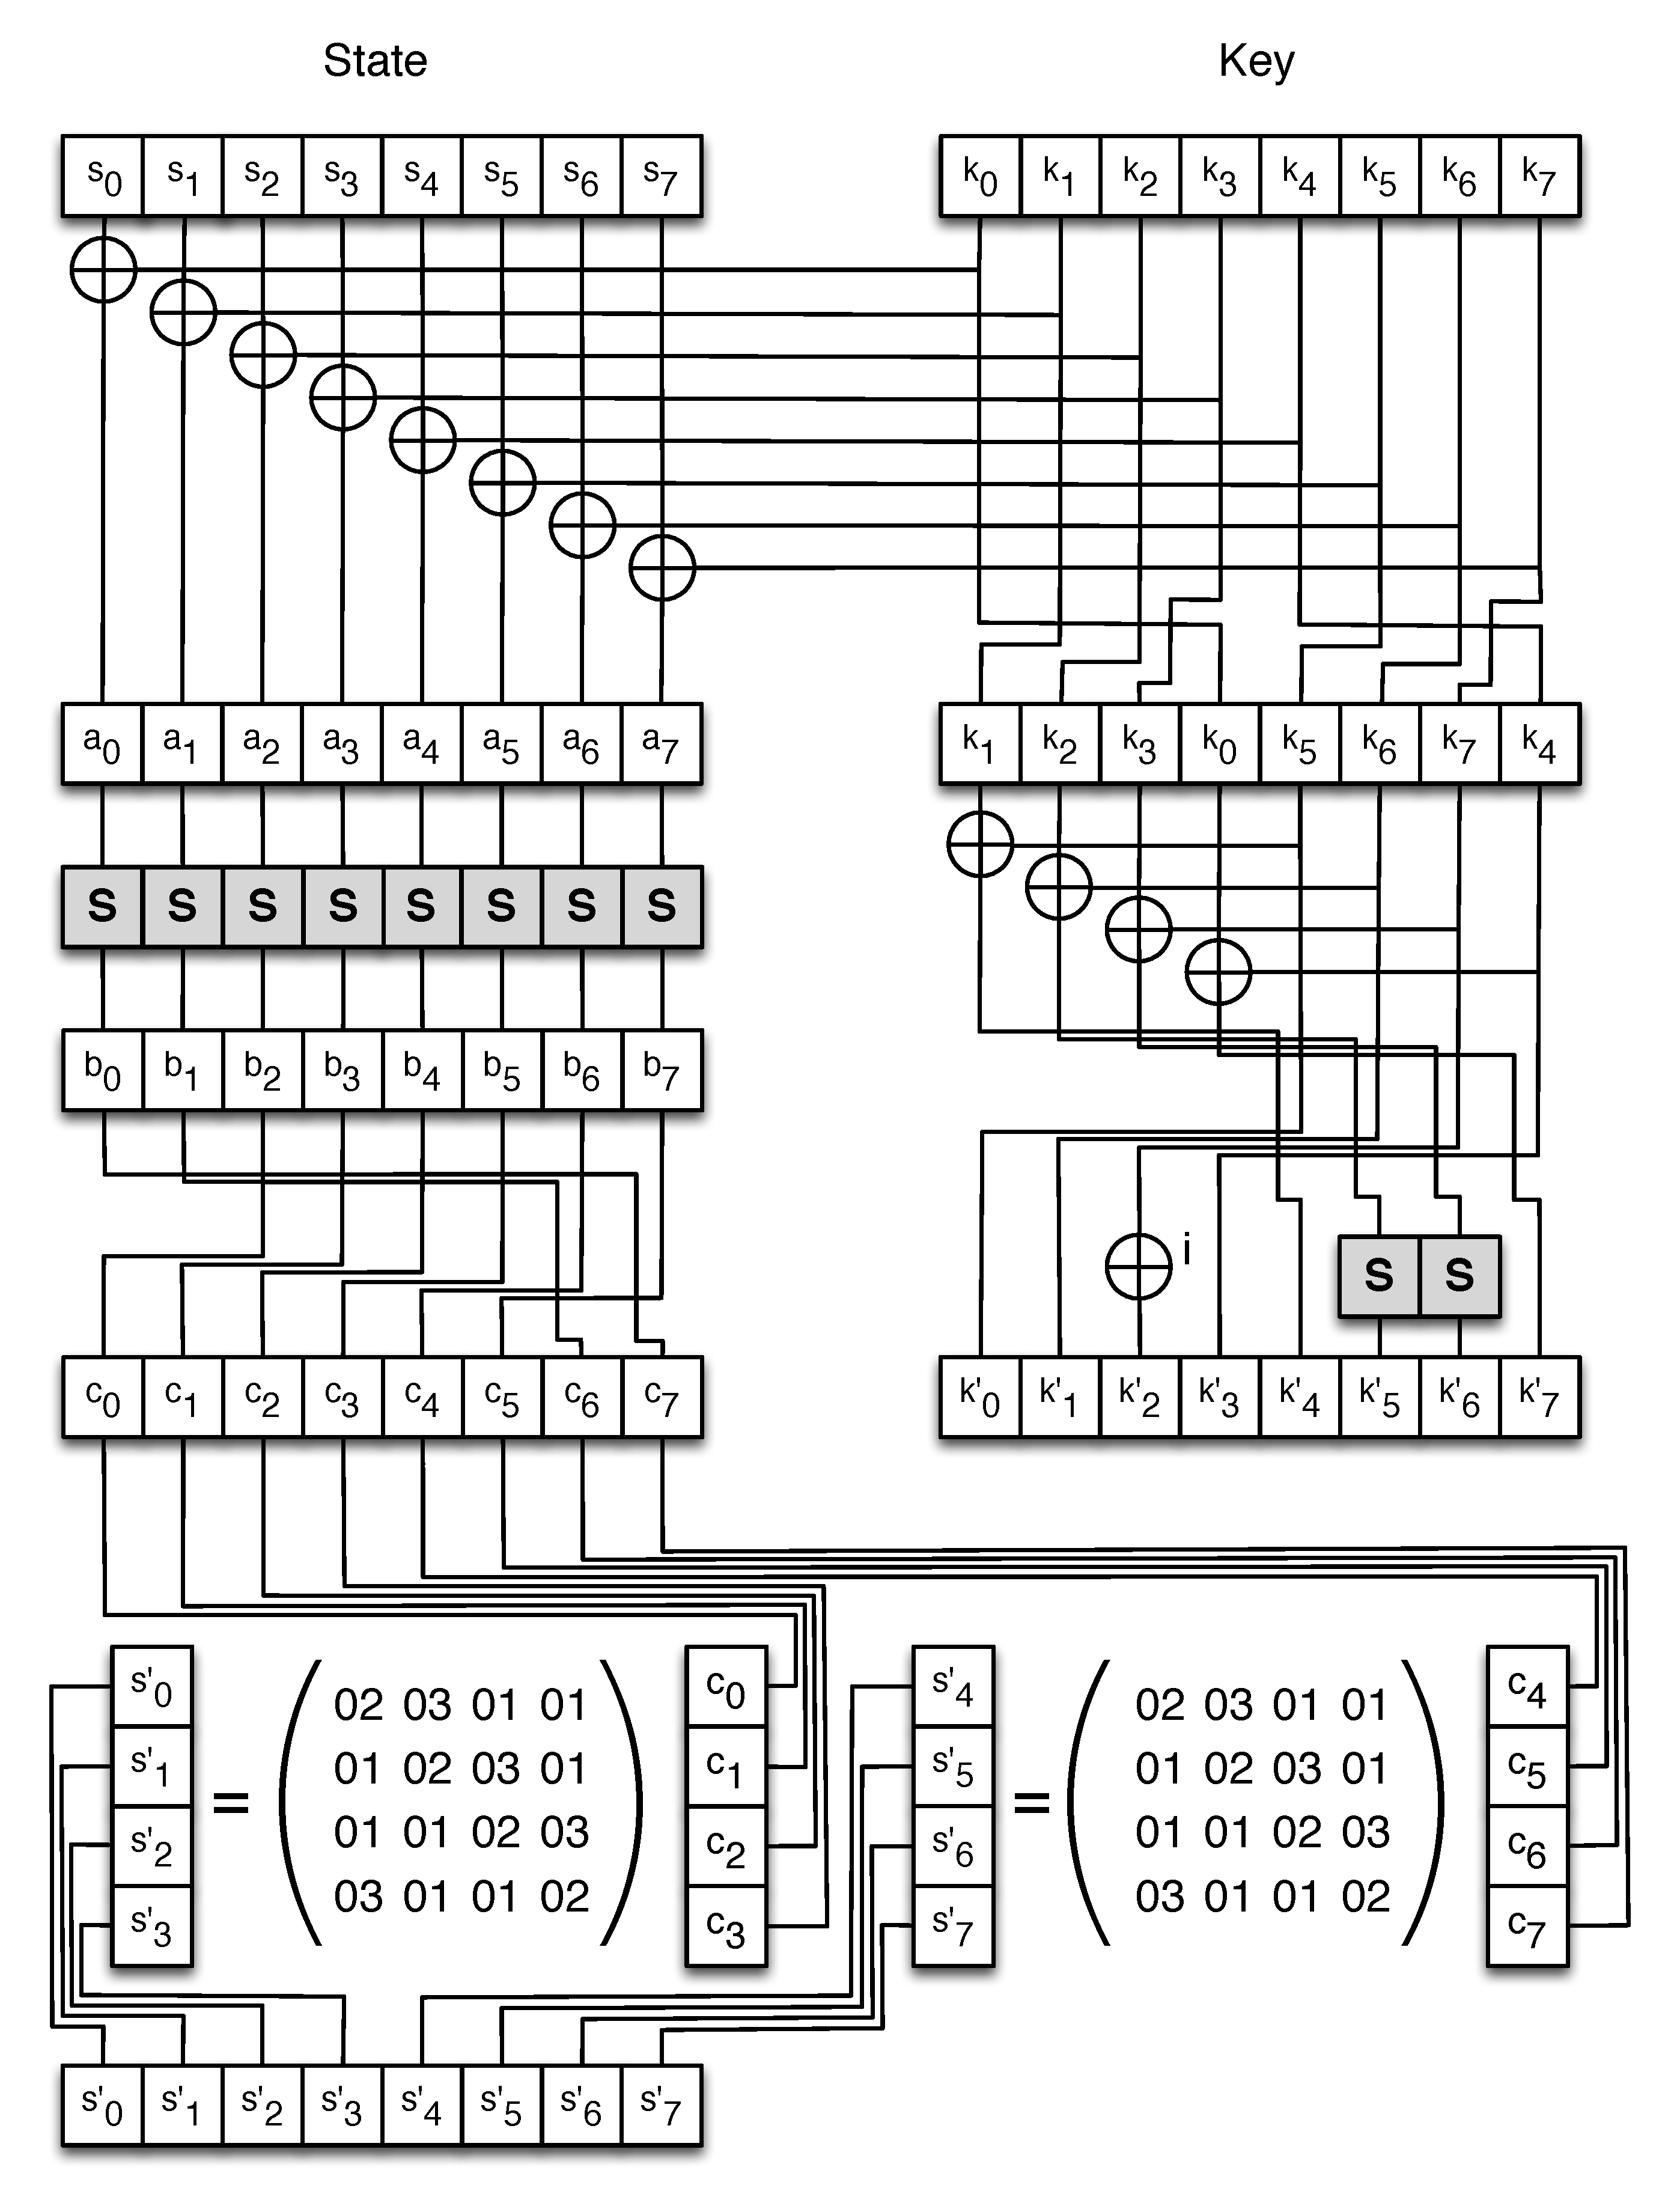
\includegraphics[scale=0.3]{diagram.pdf}}
\end{center}

\end{document}
